\section{Terrain \& Navigation}

In order to give the user the freedom to model any type of virtual world, providing the ability to specify any type of base terrain is essential. Efficient rendering and navigating this terrain is also key for both the user experience and visual realism. How our system manages these requirements are discussed sections \textit{Loading Terrain}, \textit{Rendering Terrain} and \textit{Navigating Terrain} below.

\subsection{Loading Terrain}

As stated previously, our work focuses on terrain content and not terrain relief modelling. As such, the user is only able to load a static, pre-generated terrain in the form of a Terragen height-map. A height-map is a 2-dimensional grid of height values which, once loaded and converted, represent the height of the individual terrain vertices. A Terragen height-map is a freely available and heavily used file-specification format which wraps raw height data with other important information such as base height, scale and dimensions.

\subsection{Rendering Terrain}

Once parsed, the height-map data is transferred to the GPU via a two dimensional texture for rendering. In order to better visualize the terrain relief, a Blinn–Phong shading model is used when rendering the terrain. Blinn–Phong is a popular and efficient shading model which uses a combination of camera position, light direction, surface normals, material and light color specifications to produce a visual appealing rendering which accentuates relief change.\\
Calculating the normal vectors for each point on the terrain is done using the algorithm outlined in figure \ref{fig:normals_calculation}. Each normal is calculated in parallel on the GPU, thus ensuring real-time results.

\begin{figure}[h]
\center
	\label{fig:normals_calculation}
	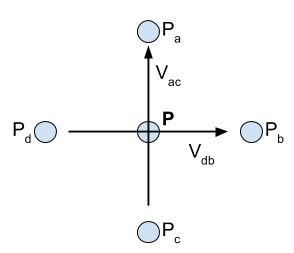
\includegraphics[width=\textwidth/2]{normals_calculation.png}
	\caption{Terrain normals calculation. $N_{P} = V_{ac} \times V_{db} $ where $N_{P}$ is the normal vector at point P and $P_{A}$, $P_{B}$, $P_{C}$ and $P_{D}$ are the direct points surrounding P in the X and Y direction. }
\end{figure}

\subsection{Navigation}

In order for users to successfully and intuitively navigate through virtual worlds, it is important to prevent any form of disorientation. Appropriate control sensitivity, logical points of references and predictable correlation between mouse movements and corresponding virtual world movements are all essential in preventing possible disorientation.\\
A point of reference in virtual worlds is a point that doesn't change and around which all other points are free to move. Two common reference points are used when visualising a virtual 3-D space: the camera or scene objects.\\
Arc-ball is a popular technique in which the camera remains static and therefore acts as the point of reference. Arc-balls are popular in modern modelling software packages and permit users to interact with scene objects through intuitive click and drag gestures.\\
Navigation techniques where scene objects act as the point of reference are most common in video games where the camera moves around a static scene. \\
Static scene with moving camera is the most widespread navigation style and the most similar to the real-world where the earth acts as the static scene and us humans act as the moving camera. In order for a more variety of users (novice to computer graphic experts) to get up to speed with the controls efficiently, this is the navigation style used in our system.\\

Two different control types can be selected which are described in more detail in table \ref{tab:control_types}: \textit{first-person} and \textit{click-and-drag}. The active control type is easily configurable, along with sensitivity parameters, through the applications settings interface. By providing multiple control-types and the ability to customise them the system can better cater to the requirements of a wider user-base.

\begin{table}[h]
  \centering
	  \label{tab:control_types}
	    \begin{tabular}{|p{3cm}|p{2.5cm}|p{2.5cm}|p{2.5cm}|p{2.5cm}|p{2.5cm}|}
  	    \hline	
  	    \textbf{Control-type} & \textbf{Translate Left/Right} & \textbf{Translate Up/Down} & \textbf{Translate Front/Back} & \textbf{Rotate Left/Right} & \textbf{Rotate Up/Down} \\
		\hline
		\textbf{First-Person} & A/D key-press & - & W/S key-press & Horizontal mouse movement & Vertical mouse movement \\
		\hline
		\textbf{Click-and-drag} & Horizontal click \& drag & Vertical click \& drag & Scroll wheel & Ctrl + horizontal click \& drag & Ctrl + vertical click \& drag\\
		\hline
		\end{tabular}
		\caption{Control types instruction sheet}
\end{table}

